\documentclass{report}
\usepackage{filecontents}

\usepackage[utf8]{inputenc}
\usepackage[T1]{fontenc}
\usepackage[francais]{babel}
\usepackage{listings}
\usepackage[a4paper]{geometry}
\usepackage{graphicx}
\usepackage[export]{adjustbox}
\usepackage{titlesec}
\usepackage{color}
\usepackage[toc, page]{appendix}
\usepackage{url}
\usepackage{pdfpages}

\lstset{frame=tb,
  language=Java,
  aboveskip=3mm,
  belowskip=3mm,
  showstringspaces=false,
  columns=flexible,
  basicstyle={\small\ttfamily},
  numbers=none,
  numberstyle=\tiny\color{gray},
  keywordstyle=\color{blue},
  commentstyle=\color{dkgreen},
  stringstyle=\color{mauve},
  breaklines=true,
  breakatwhitespace=true,
  tabsize=3
}

\definecolor{dkgreen}{rgb}{0,0.6,0}
\definecolor{gray}{rgb}{0.5,0.5,0.5}
\definecolor{mauve}{rgb}{0.58,0,0.82}
\definecolor{xcodekw}{rgb}{0.75, 0.22, 0.60}
\definecolor{xcodestr}{rgb}{0.89, 0.27, 0.30}
\definecolor{xcodecmt}{rgb}{0.31, 0.73, 0.35}

\titleformat{\chapter}[display]
  {\centering\normalfont\huge\bfseries}
  {\chaptertitlename\ \thechapter}
  {20pt}
  {\Huge}

\setcounter{secnumdepth}{5}

\titleformat{\paragraph}
{\normalfont\normalsize\bfseries}{\theparagraph}{1em}{}
\titlespacing*{\paragraph}
{0pt}{3.25ex plus 1ex minus .2ex}{1.5ex plus .2ex}

\geometry{hscale=0.75,vscale=0.85,centering}

\renewcommand{\thesection}{\arabic{section}}
\renewcommand\appendixtocname{Annexes}
\renewcommand\appendixname{Annexes}
\renewcommand\appendixpagename{Annexes}

\title{Rapport de Stage}
\author{Samuel \bsc{Monroe}}

\date{\today}

\begin{document}

\maketitle

\newpage
\thispagestyle{empty}
\mbox{}

\tableofcontents

\chapter*{Remerciements}

  Je voudrais tout d'abord remercier Virginie Van Den Schrieck et Marie-Noël Vroman, qui m'a poussé à postuler chez Belighted, pour
  le rôle qu'elles ont tenu dans le projet d'intégration du premier quadrimestre,
  en nous ayant responsabilisés quant à la gestion de notre projet et donné carte
  blanche pour la réalisation de celui-ci.
  C'est donc grâce à elles que j'ai fait mes premiers pas dans le monde du Ruby on Rails
  et du développement web moderne en général, et ainsi avoir eu l'opportunité de faire ce stage chez Belighted.\\

  Je remercie Nicolas Jacobeus, CEO de chez Belighted, de m'avoir offert cette place de stage pendant ces quinze
  semaines où j'ai énormément progressé et pu apprendre de ce métier que je veux faire plus tard, ainsi que tous les membres
  de l'équipe pour leur accueil, leurs conseils et leur aide tout au long du stage.\\

  Je voudrais également remercier Yves Delvigne, qui par son cours de programmation multimédia
  nous a inculqué les bases du développement web, et qui a donc grandement contribué
  au chemin que j'ai entrepris de suivre depuis la deuxième année.\\

  Mes remerciements vont enfin à tous les autres professeurs de l'EPHEC qui m'ont accompagné tout au long
  de ce cursus de bachelier en technologie de l'informatique et qui ont, quelle que soit la matière
  enseignée, contribué à me transmettre un panel de connaissances varié qui m'est et me sera utile pour
  le reste de ma vie. Merci donc à Christian Lambeau, Claude Masson, Michel de Vleeschouwer,Youcef Bouterfa, Arnaud Dewulf,
  Stéphane Faulkner, Véronique Leclerq, Thomas Thiry, Maxime Vanlerberghe, Jean-François Depasse, Marc Deherve et Laurent Hirsoux.\\

\chapter{Introduction}

  Point d'orgue de ces trois années de bachelier en technologie de l'informatique, la perspective de ce stage en entreprise
  est en même temps excitante, motivante, mais aussi un peu effrayante.\\
  C'est le moment où nos acquis académiques sont confrontés à la réalité du terrain, celui du premier vrai pas vers la sortie
  de classes de l'Ephec.\\

  C'est en direction de Belighted que j'ai fait ce pas, qui m'a accueilli grâce à une petite expérience déjà acquise en Ruby on Rails.\\
  Lors de nos entretiens avant le stage, l'objectif et le travail que j'allais accomplir n'étaient pas clairement définis, néanmoins il était
  très clair qu'ils seraient de contribuer à un ou plusieurs projets au sein de l'équipe en faisant évoluer les compétences que j'avais acquises.\\
  L'objectif qu'on m'a confié lors du premier jour de stage, que je décrirai plus en détail dans les pages suivantes, était de mettre sur pied un Software as a
  Service qui offrirait une gestion des avatars très simple
  à d'autres applications web, leur évitant tout besoin de mettre en place un espace de stockage dédié et d'implémenter un
  système d'avatars.\\

  Concernant mes attentes personnelles pour ce stage, j'étais en premier lieu motivé par la perspective d'apprendre un maximum
  sur le développement web. Je voulais vivre une expérience dans une PME travaillant dans le domaine, découvrir les bonnes
  pratiques suivies lors du développement ainsi que les étapes du cycle de vie d'une application web.\\
  Plus encore, je voulais avoir l'opportunité d'être très content de me lever chaque matin pour aller faire quelque chose d'agréable et de passionnant
  dans un cadre lui-même agréable.\\

  Ce rapport de stage commencera par introduire la société Belighted, je parlerai ensuite de manière assez concise du travail que j'ai accompli lors de ces quinze semaines.\\
  Ensuite viendra une explication plus précise de points techniques que j'ai rencontrés lors de ce travail et des expériences vécues au cours de celui-ci.\\


\chapter{À propos de Belighted}

  Belighted est une PME active depuis 2008 sur le marché du développement d'applications web et mobiles.\\
  L'équipe est composée d'un peu plus de dix personnes, jeunes et passionnées, toutes travaillant dans le même open-space. Tout ceci donne
  une ambiance sûrement plus proche de la startup que de l'entreprise classique.\\

  L'entreprise s'est spécialisée dans le développement en Ruby on Rails, faisant d'elle et de son équipe des experts et la plus grosse
  boîte de développement en Rails de Belgique.\\
  Cette expertise se fonde sur une recherche de la qualité, en suivant notamment des principes Agiles et par conséquent des pratiques
  telles que le développement dirigé par les tests ainsi qu'une relation proche au client.\\

  Belighted étant composée d'une demi-douzaine de développeurs, il n'y a pas pour ainsi dire de structure vraiment définie et distincte au sein du personnel. \\
  Tous sont des développeurs avec un minimum d'expérience en Ruby on Rails et JavaScript, certains étant plutôt spécialisés dans les technologies mobiles et le frontend JavaScript,
  d'autres vraiment spécialisés dans le backend de Rails. \\
  Cette diversité dans les compétences leur permet de s'entre-aider et d'apporter des solutions à des problèmes survenant sur des projets dont ils ne font pas partie, et ainsi
  accroître la connaissance globale de l'entreprise. \\

  Il y a donc tout de même une structure interne à l'entreprise. Au niveau de la direction Nicolas Jacobeus est le \textit{Chief Executive Officer} et fondateur de Belighted, accompagné
  d'Aurélien Vecchiato qui est le \textit{Chief Operating Officer}.\\
  Pour ce qui est des développeurs front-end et designers on retrouve Maxime Nguyen et Simon Henrotte. \\
  Les développeurs backend Ruby on Rails sont Philippe Van Eerdenbrugghe, Kathleen Clacens, Philippe Bourez et Dominique Lebrun.\\
  Michaël est analyste business et développeur.\\

  C'est donc Philippe Van Eerdenbrugghe qui a été chargé de m'accompagner dans la réalisation de mon SaaS, étant un développeur senior en Rails et ayant de très grandes connaissances et compétences.\\
  Il m'a énormément appris et surtout conditionné au développement dirigé par les tests et à l'application de spécifications et de bonnes pratiques dans le développement logiciel.\\

  Etant installé entre Kathleen et Philippe tout au long du stage, Kathleen a également pu m'aider sur certains points en Rails, ainsi que tous les membres de l'équipe qui m'ont conseillé et orienté sans
  hésitation lorsque j'avais la moindre question.\\


\chapter{Nature du stage et modalités de réalisation}

  Etant novice dans le développement Rails et JavaScript, Nicolas m'a confié un projet interne qui me permettrait d'une part de faire énormément progresser mes compétences dans ces domaines, et
  d'autre part de me confronter à des problèmes et à des questions que pose la conception d'un \textit{Software as a Service} pour contribuer à la connaissance de l'entreprise dans ce domaine.\\
  J'ai également été chargé de rédiger de manière régulière des \textit{blogposts}, afin de contribuer à l'activité du blog de Belighted et de partager cette expérience que j'aurais à mener.

  Ce SaaS a été nommé \textbf{Pravatar}, pour \textit{Private Avatar}, et l'idée était de développer un service qui se chargerait de toute la gestion d'avatars à la place d'applications clientes.\\
  Une application cliente désireuse d'implémenter un système d'avatars n'aurait alors plus qu'à souscrire à Pravatar, et dans l'idéal plus qu'à insérer un tag HTML \textit{<script>} pour importer un script
  JavaScript permettant la gestion des avatars.\\
  Pravatar aurait alors pu faire économiser à l'équipe un certain nombre de jours de développement par projet en matière de gestion d'avatars, mais potentiellement se vendre à d'autres applications.\\

  Ma mission était donc la suivante : \\

  \begin{itemize}
    \item Explorer dans quelles mesures un service de ce type est faisable.
    \item Mettre en lumière les contraintes rencontrées lors du développement.
    \item Apporter des éléments de solutions à ces contraintes.
    \item Au terme du stage, avoir mis sur pieds un service qui permette à Belighted de déterminer si la solution est viable, et maintenable par l'équipe si tel était le cas.
    \item Le test final était d'implémenter Pravatar sur Scale, un SaaS de resource management développé en interne par Belighted.\\
  \end{itemize}

  Je vais au long des sections qui suivent décrire de manière assez concise l'entièreté du travail accompli sur ce SaaS au cours de mon stage, les détails plus techniques et qui ont réellement contribué
  à l'entreprise seront détaillés dans le chapitre suivant.\\

  \section{Les bases du service}
  \label{sec:Les bases du service}

    \subsection{Mise en place du backend}
    \label{subs:Mise en place du backend}

      La première étape de mon travail sur Pravatar fut de mettre en place le bon environnement de travail et de poser les bases saines du backend en Ruby on Rails.\\
      Philippe, mon mentor lors du stage, en a surtout profité pour m'inculquer les bonnes pratiques à suivre et la façon dont l'équipe s'y prend pour commencer un nouveau projet.\\

      J'ai donc commencé par configurer tout l'environnement, ainsi que d'inclure un service d'administration de l'application via la gemme \textit{ActiveAdmin}.\\
      Une fois installée, j'ai pu commencer le développement de la partie administration en \textbf{Behaviour Driven Development} avec RSpec.\\

      Le but était de me former dans la démarche d'écrire des tests de features avant toute chose, écris à la manière des \textit{User Stories} propres aux méthodes Agiles, et seulement enfin
      d'écrire le code qui couvrait ces tests, suivant le cycle Red-Green-Refactor. Ce fut une vraie mise en pratique des concepts théoriques enseignés lors du cours d'intégration de Mr.Thiry.\\

      Une fois habitué à cette manière de travailler, j'ai pu commencer le développement d'une \textbf{RESTapi} sur le backend qui serait chargée de fournir les endpoints pour le script tiers
      à inclure chez les clients.\\
      Encore une fois, ce développement s'est fait dans une démarche \textit{TDD}, où j'écrivais les tests de requêtes avant même d'écrire cette API.\\

    \subsection{Le script tiers}
    \label{subs:Le script tiers}

      Les détails de conception du script ont été placés sous mon entière responsabilité, c'était justement un des points d'interrogation de Belighted au sujet de la réalisation de ce type de Software as
      a Service.\\
      Cette solution se devait d'être simple à installer et ne pas entrer en conflit avec la configuration du client, peu importe les technologies utilisées par celle-ci.\\

      J'ai donc pris le parti de développer ce script en pur JavaScript/jQuery, en faisant en sorte que ce script soit fourni avec sa propre version de jQuery afin de ne pas interférer avec une
      possible version préinstallée chez le client.\\
      Ce script était chargé de parser le code HTML présent chez le client pour y cibler des éléments comportant des \textit{data-type} spécifiques précisant l'upload ou l'affichage d'un avatar, et d'ensuite
      interagir avec mon API afin de récupérer ou mettre à jour les avatars.\\

      Philippe m'a bien évidemment chargé de mettre au point une solution de testing de ce script tiers, qui était fourni par l'application Rails mais qui existait en tant qu'élément distinct du backend.\\
      Le framework de testing \textbf{Jasmine} a fourni une solution très proche de RSpec dans la manière syntaxique d'écrire les tests, et l'utilisation de \textbf{Karma} en tant que test-runner a
      permis la gestion entière du script au sein même de l'application Rails.\\

  \section{Améliorations de Pravatar}
  \label{sec:Améliorations de Pravatar}

    Les bases du service ayant été posées et ayant pu faire fonctionner celui-ci, j'ai dû améliorer l'ensemble qui était encore relativement basique.\\

    \subsection{Améliorations du backend}
    \label{subs:Améliorations du backend}

      La première amélioration a consisté en l'insertion d'une quatrième couche à l'architecture MVC. En effet, la tendance d'un débutant en Rails est de surcharger la responsabilité des contrôleurs, alors qu'en
      principe un contrôleur n'est chargé que de récupérer une ressource et de répondre à une requête avec celle-ci.\\
      La phrase Rails visant à pallier à ce problème annonce \textit{"Fat models, skinny controllers"}.\\
      La surcharge des modèles n'est en réalité pas la meilleure façon qui soit de concevoir l'application, et c'est pour cela que j'ai été chargé par Philippe d'insérer des \textbf{interacteurs}, qui sont des
      objets chargés d'encapsuler la logique business d'une application, et de laisser aux contrôleurs la façon spécifique de répondre aux requêtes.\\

      J'ai dû ensuite mettre en place du stockage des images sur une instance Amazon S3.\\
      Cette configuration du stockage Amazon S3 est justement ce que Pravatar devrait absorber sur les autres projets de chez Belighted.\\

      Une importante mise à jour du service fut sa mise en conformité par rapport à la spécification \textit{JSON:API}. En effet, une API JSON peut en pratique répondre ou recevoir des requêtes
      comportant n'importe quelle structure JSON.\\
      Cette liberté peut néanmoins se révéler problématique selon la vision des développeurs quant à la définition des ressources qui doivent être échangées sur cette API.\\
      J'ai donc dû transformer celle de Pravatar afin de suivre la spécification JSON:API, qui précise une manière "standard" de représenter ces ressources.\\

    \subsection{Améliorations du front-end}
    \label{sub:Améliorations du front-end}

      Au fur et à mesure du développement du script tiers, travaillant avec du Javacript pur, je me suis rapidement retrouvé avec un amas de fonctions difficilement maintenables.\\
      J'ai pu grâce à \textbf{Browerify} opérer une découpe de mon code en modules indépendants et définis selon leurs responsabilités.\\
      Le code du script est devenu beaucoup plus compréhensible, et évidemment beaucoup plus maintenable du fait de cette découpe en modules.\\
      Une réécriture du code en Coffeescript m'a également été demandée par Philippe.

      Suite à cette réécriture en Coffeescript et à l'indépendance de l'environnement du script, la compilation et le packaging de celui-ci n'étaient évidemment plus assurés par l'asset pipeline de Rails.\\
      J'ai donc pu mettre en place un système d'automatisation de compilation et de configuration avec l'outil \textbf{Gulp}, ce qui a permis un travail fluide sur le script
      plus ou moins comme on aurait travaillé sur Rails.\\
      Ceci était impératif, puisque le script devait résider au sein du projet Rails, mais vivre dans son propre écosystème.\\

    \subsection{Gem}
    \label{sub:Gem}

      Afin de faciliter l'implémentation du service sur des projets Ruby on Rails, j'ai entamé le projet de créer une gem qui pourrait être incluse dans les projets clients et qui rendrait le service
      extrêmement facile à mettre en place.\\

      Cette gem était un \textbf{engine} Rails, fournissant à l'application deux méthodes très simples et concises afin de déclarer soit l'affichage d'un avatar, soit la définition d'une zone d'upload pour
      mettre à jour l'avatar.\\
      Le code HTML généré par ces méthodes était personnalisable via des générateurs, qui dupliquaient les templates fournis par la gemme chez le client et l'autorisaient à totalement modifier le rendu.\\

    \subsection{Sécurité}
    \label{sub:Sécurité}

      A ce stade avancé du projet, la question de la sécurité du système des avatars s'est posée. Il fallait pouvoir empêcher des uploads non désirés sur Pravatar.\\
      Cette sécurisation a été accomplie via l'utilisation de \textbf{JSON Web Token}, qui permet une signature de données JSON via une clé secrète et est décrite dans la \textit{RFC 7519}.

  \section{Finalisation du projet}
  \label{sec:Finalisation du projet}


    \subsection{Fin du développement}
    \label{sub:Fin du développement}

      Afin de pouvoir tester mon travail avec le backend, le script et la gemme, j'ai créé un petit projet Rails dans l'unique but d'implémenter le service Pravatar.\\
      L'utilisation de la gem et du script s'est révélée être extrêmement simple, et le tout fonctionnait très bien.\\

      L'étape finale de la mise à l'épreuve de Pravatar fut son implémentation sur Scale, un des projets internes de chez Belighted.\\
      Scale fonctionnant avec un stack AngularJS/Rails, je me suis rapidement retrouvé dans l'impossibilité d'utiliser la gemme et le script sur ce projet à cause de la single-page app écrite en Angular.\\
      J'ai donc eu l'opportunité d'apprendre AngularJS et de commencer l'implémentation du service en pur Angular en utilisant l'API de Pravatar.\\
      Le résultat final s'est avéré vraiment gratifiant pour ma part, me lancer dans une nouvelle technologie telle qu'Angular n'ayant pas été forcément très facile dès le début.\\

    \subsection{Dernier travaux}
    \label{sub:Dernier travaux}

      Les derniers jours de mon travail au sein de l'entreprise ont consisté en la rédaction de mon compte-rendu sur les découvertes et éléments importants que j'avais pu retirer de cette expérience,
      et qui étaient très importants pour Belighted et pour leurs futurs travaux sur des SaaS.


\chapter{Expériences vécues et objet d'étude}

  \section{Expériences vécues au sein de Belighted}

    D'un naturel assez timide et réservé, j'espère et j'estime cependant m'être assez bien intégré au sein de l'équipe de chez Belighted.\\

    Au niveau des relations avec les collègues, j'étais principalement en contact avec Kathleen et Philippe puisque je travaillais entre eux deux, mais j'ai pu également pas mal discuter avec
    l'ensemble de l'équipe, que ce soit à propos de sujets techniques ou totalement personnels.\\

    Chaque lundi midi se tenait un \textit{weekly}, sorte de stand-up meeting, mais où toute l'équipe se réunissait pour manger et où chacun parlait de ce qu'il faisait actuellement.\\
    Je pense que ce weekly était surtout utile pour Nicolas afin qu'il ait une vision globale d'où en étaient tous les projets.\\
    De vrais stand-up meetings me semblaient difficiles à tenir puisque maximum deux employés travaillaient sur le même projet en même temps.\\

    J'ai eu aussi l'occasion d'aller manger à l'extérieur avec l'équipe, faire une sortie badminton, mais aussi d'aller quelques fois boire un verre hors des heures de bureau une fois la journée terminée.\\
    C'était vraiment agréable et je ne sais pas si j'aurais pu avoir l'occasion de faire ce genre de choses dans une plus grosse entreprise.\\

  \section{Compte rendu sur l'expérience du développement d'un SaaS}
  \label{sec:Compte rendu sur l'expérience du développement d'un SaaS}

    Ce compte-rendu de mon expérience reprend avec plus de détails tous les éléments de réponses et découvertes qui seront utiles à l'entreprise suite à l'accomplissement du projet Pravatar.\\

    \subsection{Création d'un script tiers en pur JS/jQuery}
    \label{sub:Création d'un script tiers en pur JS/jQuery}

      Le premier challenge du service Pravatar était le suivant :\\
      \textit{"Comment créer un third-party widget à intégrer dans d'autres applications pour utiliser le service de Pravatar, sans altérer la configuration du client?"}\\

      La solution qui présentait le moins de contraintes et également l'approche la plus simple pour moi s'est avérée celle de créer un snippet \textbf{JavaScript} important
      sa propre version de \textbf{jQuery}, de sorte qu'il n'interfère en aucun cas avec l'application du client peu importe sa configuration.\\

        \subsubsection{Browserify}
        \label{subs:Browserify}

          jQuery ayant été sélectionné pour accomplir le travail d'échange avec Pravatar, et donc d'affichage et d'upload chez le client, la question de \textbf{conflit} de version s'est posée.\\

          \textbf{Browserify} couvrait cette question en proposant l'option de packager des éléments JavaScript entre eux afin d'en ressortir un
          \textit{bundle} indépendant des technologies présentes chez le client.\\

          Ceci a permis via un système de "require()", de spécifier le requirement de jQuery dans le snippet et donc de l'intégrer dans une application cliente de
          manière transparente et non conflictuelle.\\


          JavaScript tel quel ne propose pas réellement de solution pour séparer le code selon les \textbf{responsabilités} couvertes.\\
          Du fait de mon expérience un peu trop fraîche sur le JavaScript au moment de créer ce script, celui-ci est rapidement
          devenu un gros fichier plein de fonctions s'appelant les unes les autres et dont les liens devenaient un peu difficiles à identifier.\\

          J'étais cependant passé à côté d'un avantage qu'offrait \textbf{Browserify} et que j'aurais pu utiliser afin de régler ce problème.\\

          Le système de requiremenents fourni par Browserify pour intégrer d'autres librairies au script peut aussi être utilisé au sein du
          script lui-même pour décomposer le code et créer un arbre logique de sous-composants selon leurs \textbf{dépendances} et \textbf{responsabilités}.\\
          Cette décomposition force une certaine rigueur dans le développement de ces composants, d'autant que deux composants qui se "require()"
          mutuellement provoquent une dépendance circulaire empêchant le code de fonctionner.\\

          Enfin, encore un avantage proposé par cette décomposition en \textbf{sous-modules} via Browserify était lié au testing.\\
          En effet, certains éléments concernant le drag'n'drop des images pour upload aurait été extrêmement compliqués à tester.\\
          Cependant, en incluant le sous-module responsable de l'upload via un require() dans le test associé, il était possible de tester de
          manière isolée l'upload d'une image, que celle-ci soit faite en drag'n'drop ou via un file input.\\

        \subsubsection{Utilisation du script chez le client}
        \label{subs:Utilisation du script chez le client}

          Le script étant bundlé et prêt à l'emploi, les options d'exécution du code chez le client n'étaient pas innombrables.\\

          Les options qui ont été trouvées pour ce faire sont les suivantes :\\

          \begin{itemize}
            \item Attacher à l'objet "window", un objet "pravatar" qui expose les fonctions utilisables par le client pour générer l'affichage et l'upload des avatars.
            \item Paramétrer le lancement des fonctions sur l'évènement \$document.ready() afin de parser la page et générer les éléments dans le DOM.\\
          \end{itemize}

          La solution de l'évènement "ready" s'est avérée relativement fonctionnelle sur une application pure Rails stateless, où les actions rafraîchissaient
          la page et accomplissaient bien le travail attendu.\\

          Dans l'implémentation de Pravatar sur Scale, l'utilisation du script s'est révélée \textbf{impossible}, une implémentation directe en Angular utilisant les
          entrées d'API sur service Pravatar était beaucoup plus efficace et élégante.\\

      \subsection{Testing du script tiers fourni par Rails}
      \label{sub:Testing du script tiers fournit par Rails}

        La mise en place d'une solution de testing pour ce snippet JavaScript fourni par l'application Rails de Pravatar était indispensable.\\

        \subsubsection{Jasmine et RSpec}
        \label{subs:Jasmine et RSpec}

          Étant donné la syntaxe type scénario utilisée pour tester l'application Rails avec RSpec, il fallait dans une optique de consistance construire l'environnement de test JavaScript sur cette même syntaxe.

          \textbf{Jasmine} s'est avéré être un très bon framework de test pour ce but, et permet d'avoir des déclarations de tests qui suivent ce schéma :\\

          \begin{lstlisting}
          describe("A suite", function() {
            it("contains spec with an expectation", function() {
              expect(true).toBe(true);
            });
          });
          \end{lstlisting}

          Un autre gros avantage de Jasmine est la possibilité de lui lier des modules de testing pour assurer des fonctionnalités plus spécialisées.\\
          Dans le cas du snippet de chez Pravatar, les fonctionnalités à tester étaient principalement liées au \textbf{jQuery}.\\
          L'inclusion du package jasmine-jquery a grandement couvert ce besoin en fournissant des matchers tels que toBeChecked(), grandement utiles pour tester les changements dans le DOM.\\

        \subsubsection{Test Runner : Karma}
        \label{subs:Test Runner : Karma}

          Une fois le framework de test sélectionné, il fallait un moyen de pouvoir faire tourner ces tests Jasmine au sein du projet.\\

          Le script étant réellement une fonctionnalité séparée de l'application Rails, le test runner devait également vivre dans son propre éco-système au sein du projet.\\

          Installé via npm, \textit{Karma} est un test runner qui va exécuter les tests Jasmine sur un browser spécifié dans la configuration.\\
          De nombreuses options de configurations peuvent être paramétrées sur Karma, c'est là également que se retrouvent listés les autres modules dont les tests dépendent, tels que jasmine-jquery.\\

      \subsection{Automatisation des tâches sur le script client}
      \label{subs:Automatisation des tâches sur le script client}

        En plaçant l'environnement du script client dans son propre écosystème au sein de l'application Rails, un autre problème a dû être résolu.\\

        En effet, les sous-modules du script ayant été réécrits en \textbf{Coffeescript}, ils n'étaient plus servis et donc compilés par l'asset pipeline de Rails.\\
        Un moyen était donc nécessaire pour pouvoir travailler confortablement sur ce script, sans devoir à chaque fois recompiler le tout et relancer les tests manuellement,
        ce qui aurait été un gros frein au développement du script.\\

        Ce moyen s'est avéré être \textbf{Gulp}.\\
        Gulp m'a permis d'automatiser ces tâches de compilation/testing en créant des tâches gulp qui résument en une commande une série d'actions à effectuer.\\
        Le fichier Gulp de Pravatar permet de :\\

        \begin{itemize}
          \item Lancer les tests une fois, ou en mode surveillance à chaque changement des sources
          \item Lancer la compilation et le bundling des sources en une fois, ou également en mode surveillance afin de ne pas devoir relancer celle-ci à chaque changement dans le code.\\
        \end{itemize}

        Gulp a donné un moyen de travailler dans un worklow très proche de celui de Rails, où les tests sont aisément lancés et où il n'est pas nécessaire de déporter
        son attention du code pour continuer le travail.\\

      \subsection{Signature de données échangées via l'API}
      \label{sub:Signature de données échangées via l'API}

        Il a fallu un moment donné se pencher sur la question de la sécurité à propos de Pravatar.\\
        Comment empêcher un utilisateur de modifier les valeurs du formulaire d'upload, afin de par exemple modifier l'avatar d'un autre utilisateur?\\

        \subsubsection{Solution maison}
        \label{subs:Solution maison}

          Ma première réaction a été d'imaginer un système de sécurité "maison".\\

          Ce système de sécurité ajoutait aux \textit{params} de la requête un payload de sécurité garantissant la validité de l'upload, il était établi de la manière suivante.\\

          Au niveau client:\\

          \begin{itemize}
            \item Un hash était créé en chiffrant les données utiles via OpenSSL en utilisant l'API key du projet associé.
            \item Un digest base64 était ensuite généré à partir du hash, et placé au côté des données utiles avant envoi au serveur.\\
          \end{itemize}

          Au niveau serveur:\\

          \begin{itemize}
            \item Le digest en base64 était décodé.
            \item Un hash était recréé à partir des données en clair.
            \item Le hash reçu était comparé à celui recréé pour validation.\\
          \end{itemize}

          Ce système, bien que fonctionnel, était extrêmement lourd et rien ne me permettait d'affirmer l'inviolabilité de mon système.\\
          De plus le chiffrement via OpenSSL était complètement inutile.\\

        \subsubsection{JWT, la bonne solution}
        \label{subs:JWT, la bonne solution}

          Rétrospectivement, j'avais mal évalué les réels besoins du système de sécurité à implémenter.\\

          L'\textbf{essentiel} du problème était uniquement de s'assurer que:\\

          \begin{itemize}
            \item L'upload ne doit pas être rejouable par un utilisateur.
            \item L'utilisateur ne peut pas cibler un autre en modifiant les données d'upload.\\
          \end{itemize}

          L'url de l'API indique de toute façon l'id du profil et le nom du projet, et les données échangées n'ont absolument rien de \textit{confidentiel}.\\

          Le système de \textbf{JSON Web Token} permet de créer un ensemble de données comprenant un \textbf{header}, le \textbf{payload}
          avec les données utiles et une \textbf{vérification de signature}.\\
          Ce système permet d'échanger des données signées avec une clé, et la signature prouve qu'aucune donnée n'a été altérée.\\

          Les avantages à utiliser JWT au lieu d'une solution customisée sur Pravatar étaient les suivants :\\

          \begin{itemize}
            \item JWT est décrit dans la RFC 7519 et est donc standardisé et ouvert, inutile d'élaborer
          un système de signature incertain et lourd.
            \item La complexité du code de l'upload sur l'API a été considérablement réduite, l'encodage/décodage se fait via une simple instruction.
          Un décodage échouera sur la moindre donnée altérée et déclenchera une erreur, simplifiant encore l'implémentation.\\
          \end{itemize}

      \subsection{Communication entre l'app cliente et Pravatar}
      \label{sub:Communication entre l'app cliente et Pravatar}

        Par défaut Rails empêchait l'intervention du third-party widget sur son API.\\

        Le problème était lié aux CORS (Cross-origin resource sharing), les requêtes provenant d'un autre domaine
        que celui de l'app Rails étaient tout simplement refusées.\\

        Ceci a été réglé via la mise en place de la gem rack-cors et en spécifiant dans le fichier de configuration
        application.rb les méthodes HTTP autorisées ainsi que les origines autorisées.\\

      \subsection{Conclusion de l'expérience}
      \label{sub:Conclusion}

        La conclusion qui est ressortie au terme de ce travail sur Pravatar était que ce SaaS demanderait peut-être plus de jours/homme à être maintenu que ceux qu'il
        ferait économiser sur les divers projets.\\

        Un gros problème pour les applications JavaScripts était que la clé API posait des soucis de sécurité, en effet sur Scale, un provider Pravatar était initialisé avec la clé
        API et était forcément visible dans les fichiers sources reçus par le client.\\

        Cependant, le service pourrait avoir un intérêt réel pour sa mise en place chez d'autres clients.\\


\chapter{Conclusion}

  Je suis très heureux d'avoir eu l'opportunité de faire mon stage au sein de l'équipe de chez Belighted.\\

  Tout au long de ces quinze semaines, j'ai énormément appris et fait progresser mes compétences dans le développement web.\\
  Je peux le constater rien qu'en regardant à nouveau notre premier projet en Rails accompli pour le cours d'intégration des technologies.\\

  Je ressors de cette aventure avec des compétences que j'avais avant le stage beaucoup plus affûtées, mais également avec des tas de nouvelles autres.\\
  Cette expérience aura également été l'accomplissement pratique de nombreux concepts théoriques qui m'ont été donnés lors de cours au sein de l'Ephec, ne serait-ce qu'en
  matière de méthodologie Agile et de toutes les bonnes pratiques que celle-ci met en avant.\\

  Ce stage conclut ma troisième année de bachelier à l'Ephec m'aura apporté énormément et me conforte plus encore dans l'idée du chemin que je veux poursuivre.\\

\chapter*{Annexes}

    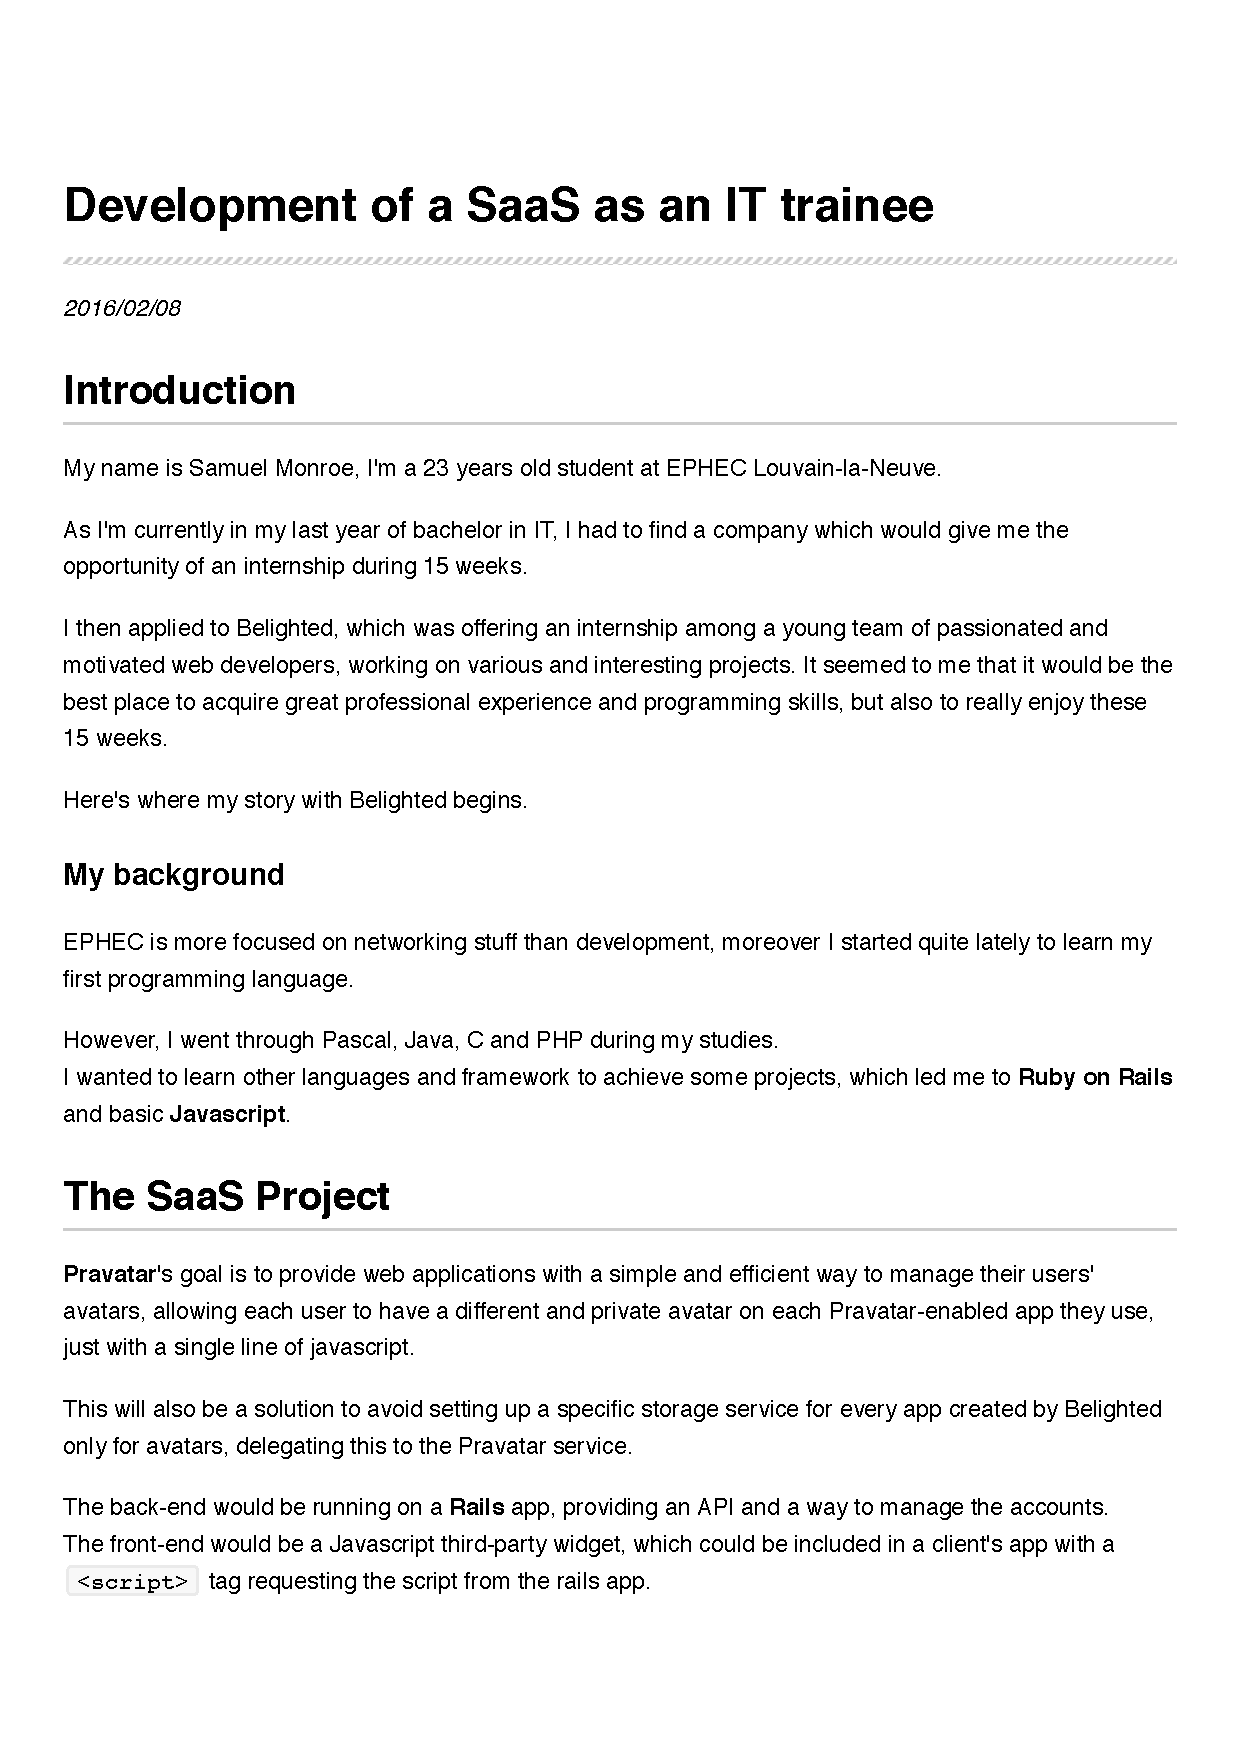
\includepdf[pages={-}]{blog_post_1.pdf}

    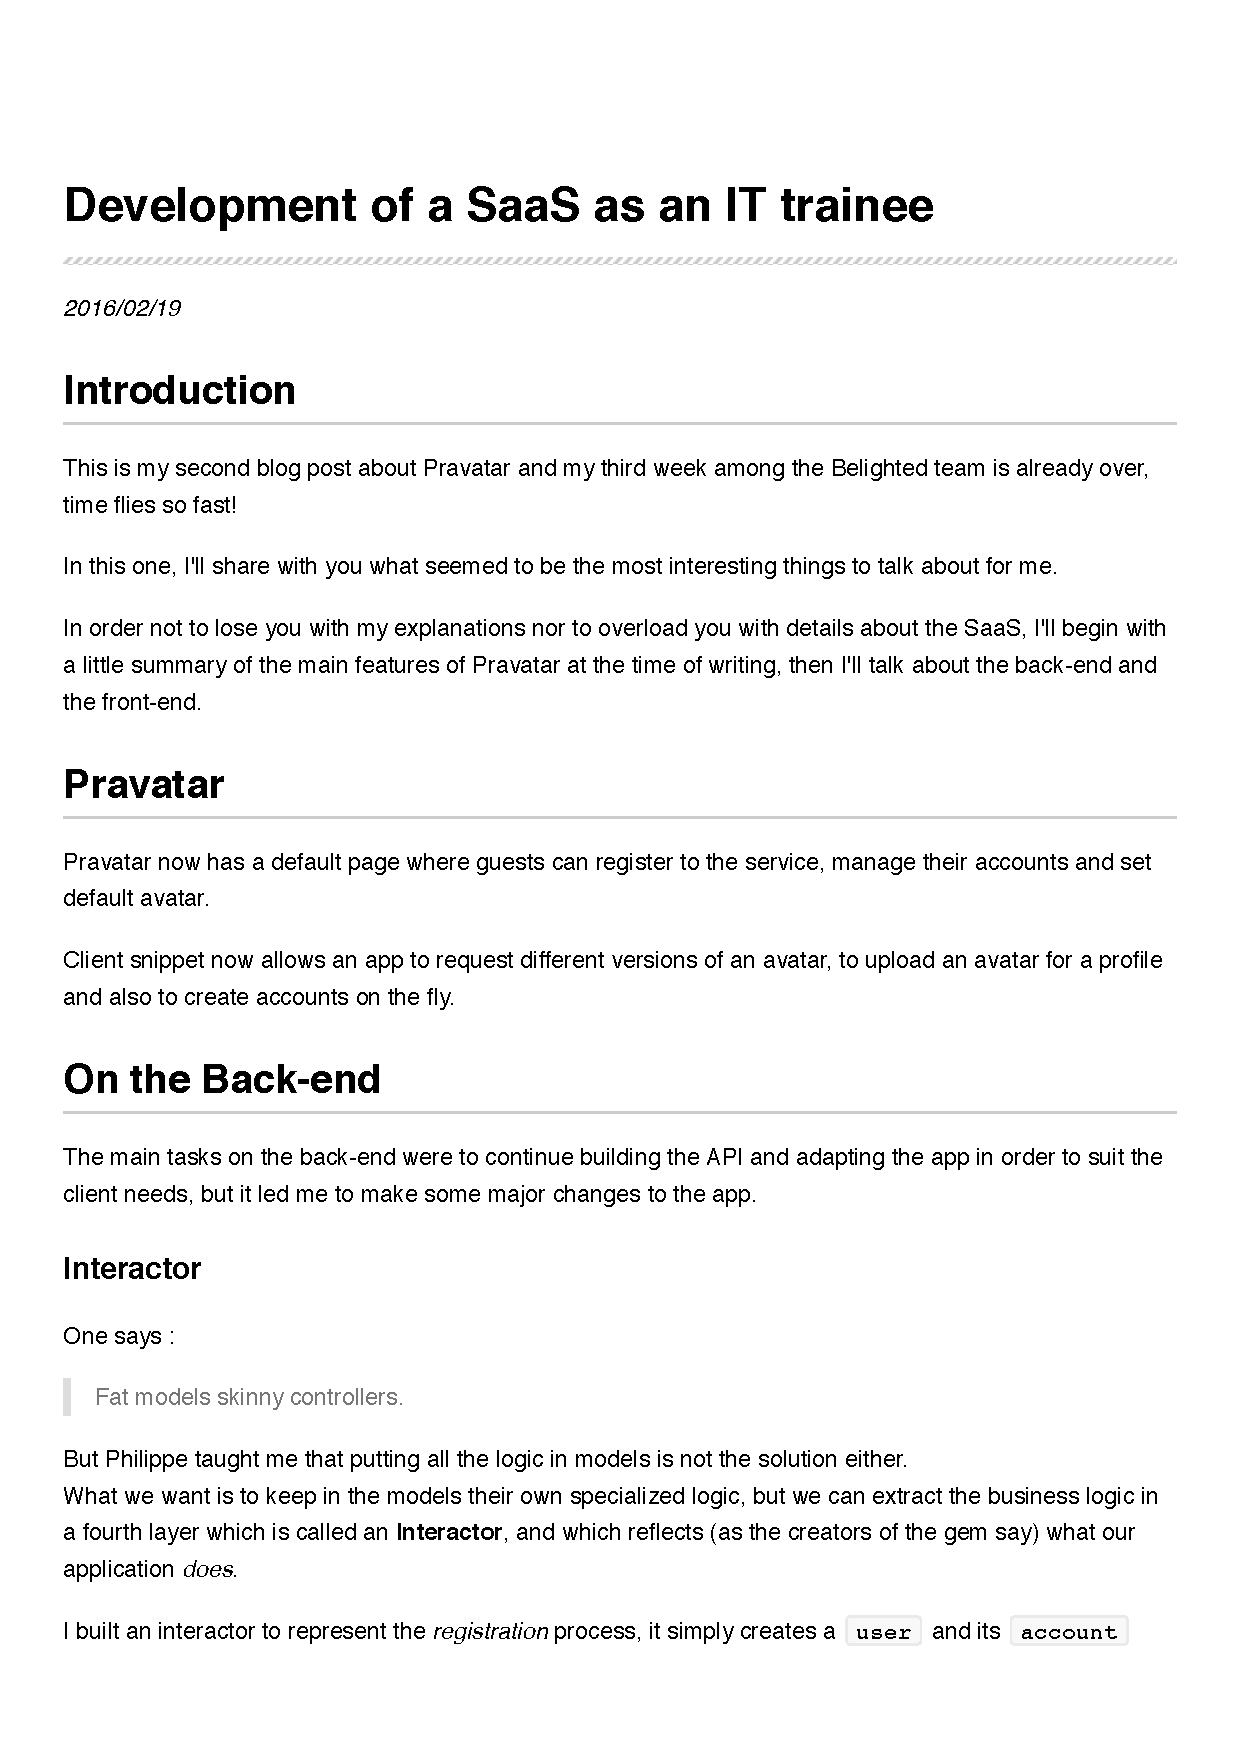
\includepdf[pages={-}]{blog_post_2.pdf}

    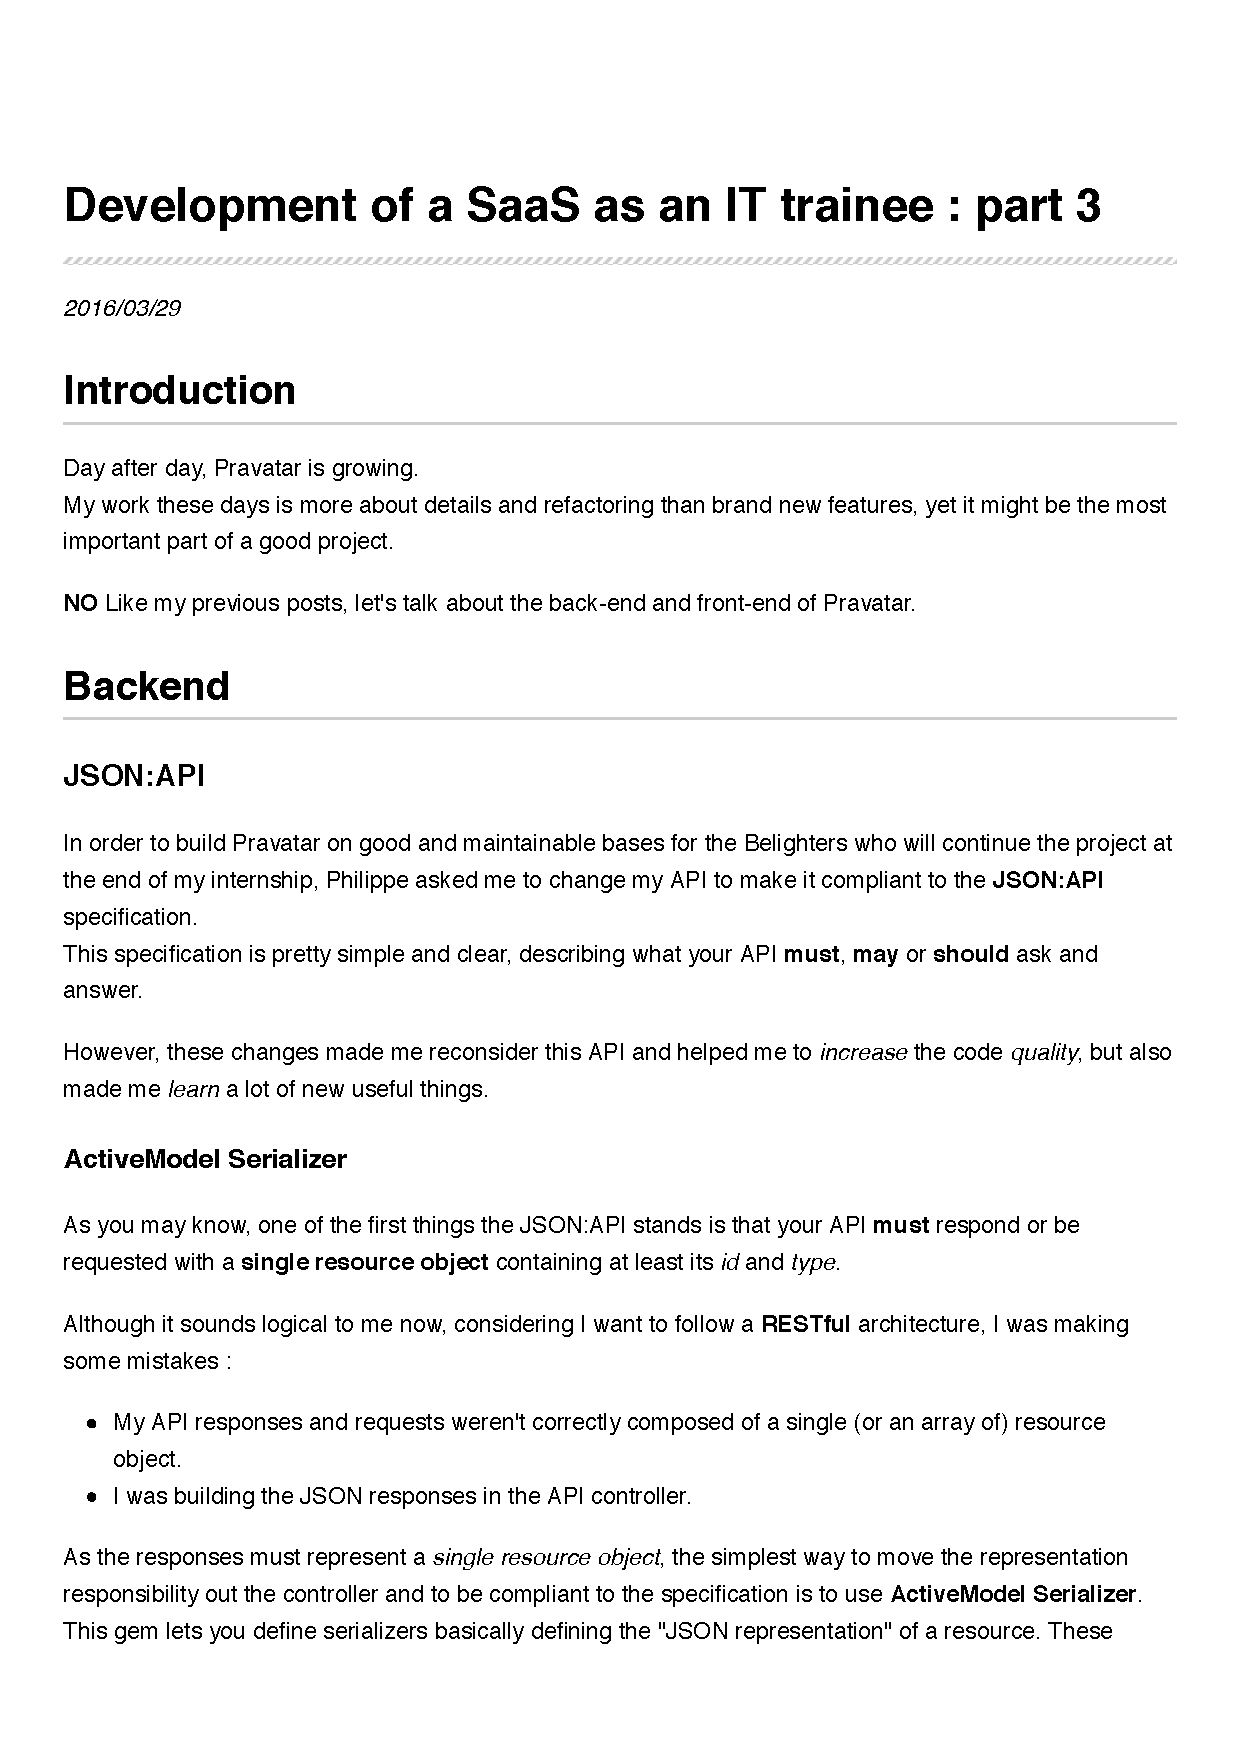
\includepdf[pages={-}]{blog_post_3.pdf}

    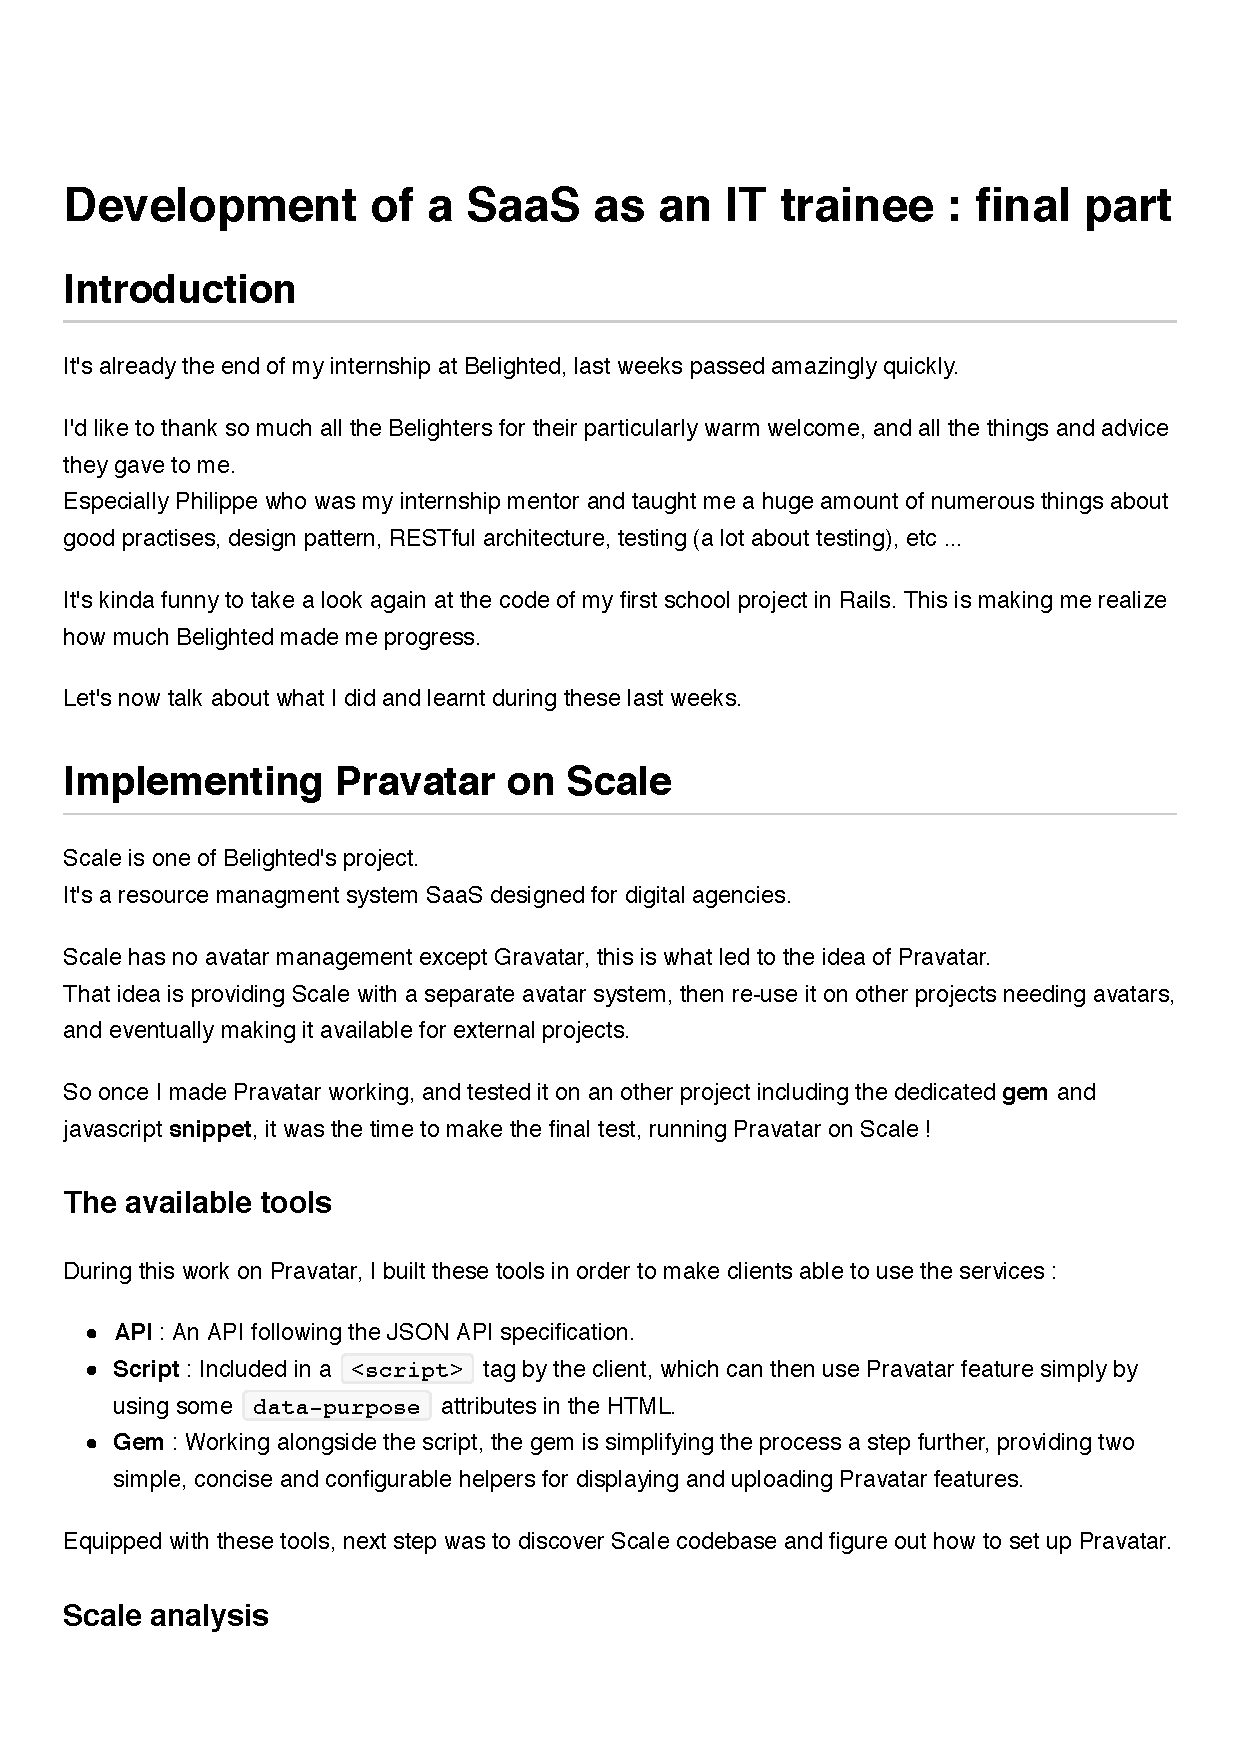
\includepdf[pages={-}]{blog_post_4.pdf}

    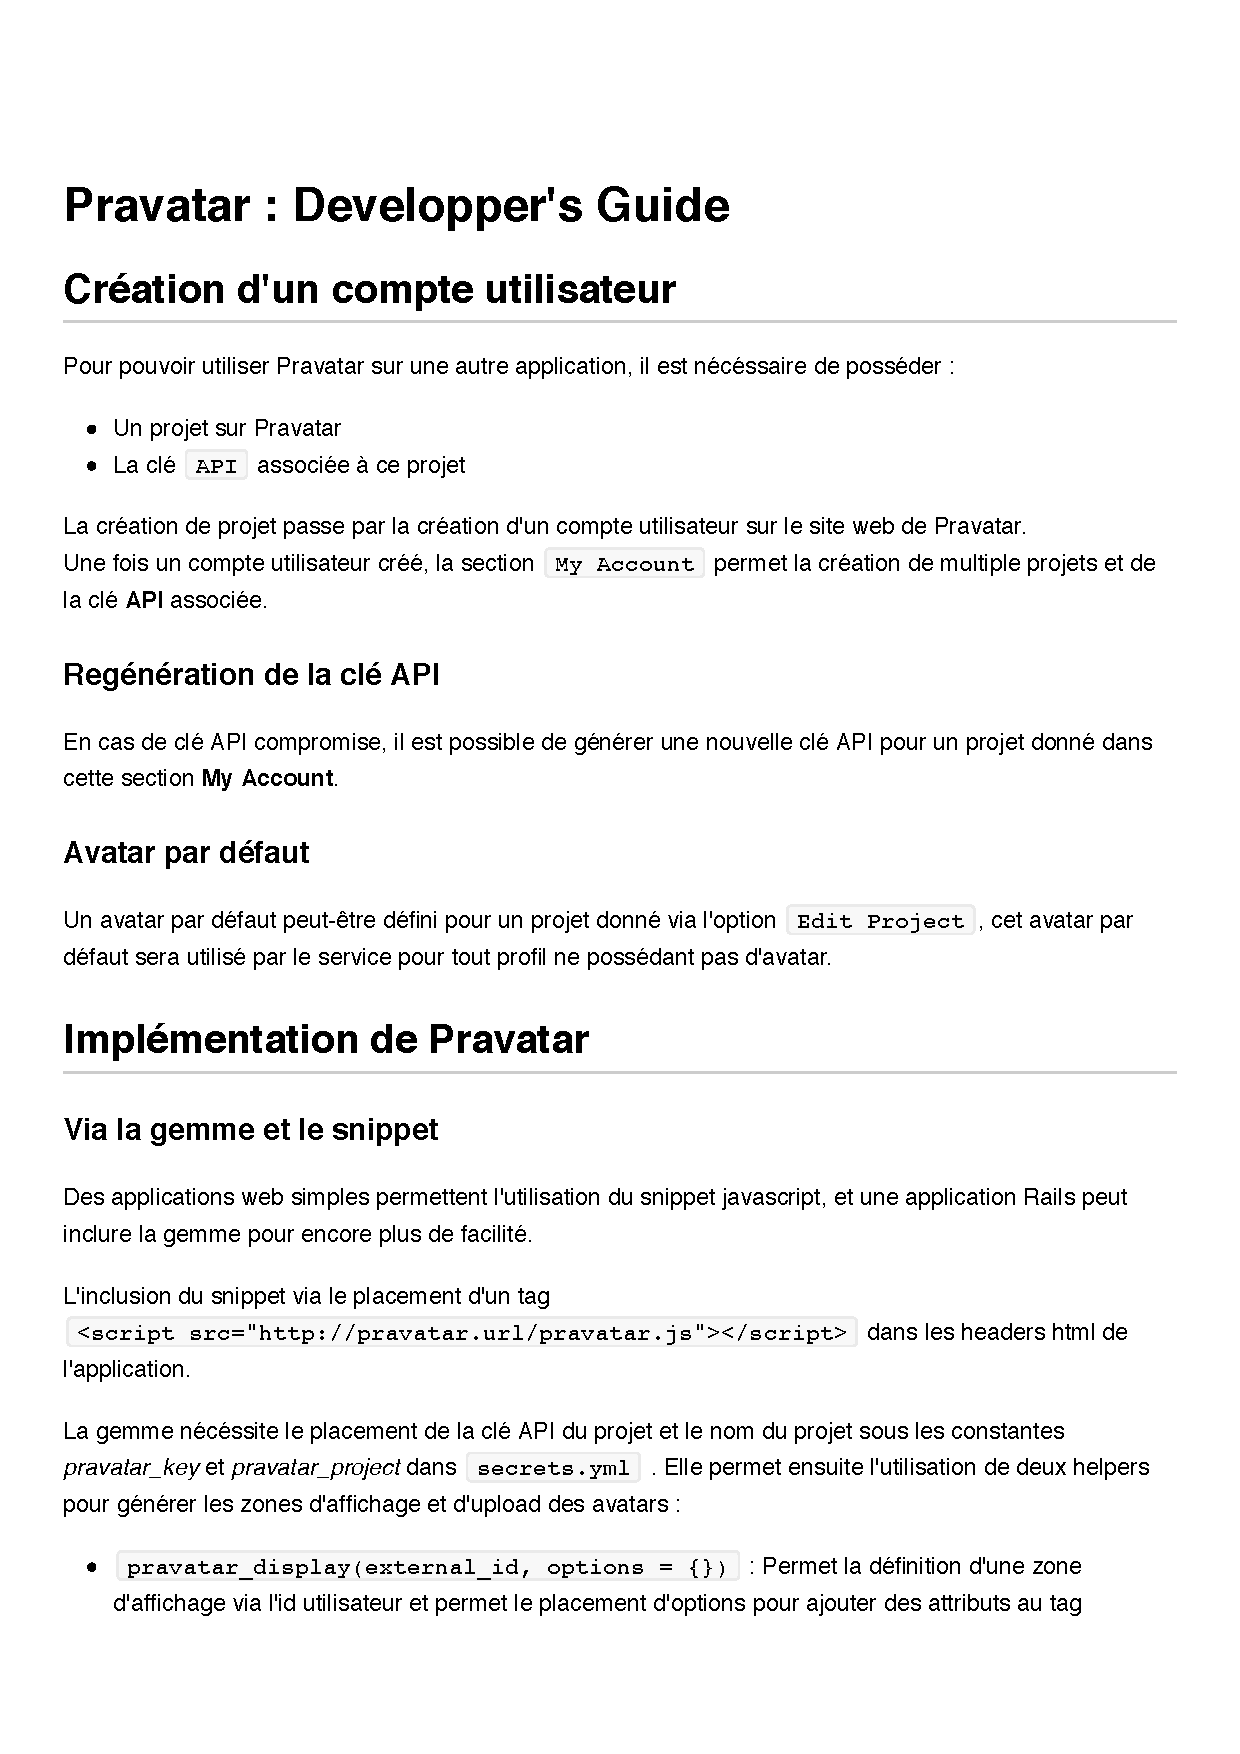
\includepdf[pages={-}]{pravatar_dev_guide.pdf}

\end{document}
